\chapter{Background}

\section{Introduction to Fuzzing}

\textit{Fuzzing}, or \textit{fuzz testing}, is a software testing technique that includes feeding a huge amount of random data into the system, called \textit{SUT (System Under Test)}, to find unprecedented responses and reveal major programming errors, along with key security vulnerabilities. The primary objective of fuzzing is to identify vulnerabilities such as \textit{buffer overflows}, \textit{memory leaks} and other security weaknesses that can be exploited by attackers (\cite{fuzzingprogresschallenges}).
\\The success of fuzzing is based on its capabilities for automatic test case generation and for focusing its attention on portions of programs that otherwise would not have been tested by other more traditional testing technique.
\\Indeed, it is particularly effective for applications with complex input grammars, where manual test case creation would be impracticable.

\subsection{Types of Fuzzing Techniques}
Fuzzing methodologies vary and there exist a lot for different applications and purposes (\textit{Fuzzers for Stateful Systems} \cite{statefulfuzzingcristian}):

\begin{itemize}
    \item \textbf{Black-box Fuzzing}: This is a technique of generating inputs without prior knowledge of the internal structure of an application. It is easy to deploy but often less efficient as there is no internal feedback.
    
    \item \textbf{White-box Fuzzing}: This is one of those techniques that rely heavily on source code intuition, such as control flow and data flow, to provide maximum \textit{code coverage} with test case generation. The approach often employs some sort of complex static and dynamic analysis methodologies.
    
    \item \textbf{Grey-box Fuzzing}: It is a strategy that combines the various merits of \textit{black-box} and \textit{white-box fuzzing}. It brings in partial knowledge about internal application details and code coverage feedback guiding the generation of inputs. It balances simplicity with effectiveness and an example might be the \textbf{AFL} tool (\textit{American Fuzzy Lop}).
\end{itemize}

\subsection{Fuzzing Inputs Generation}
There are also different ways to generate inputs for fuzzing:
\begin{itemize}
    \item \textbf{Mutation-based Fuzzing}: This generates new inputs through random mutations of existing inputs (for example modifying bits or bytes of existing test cases). It requires no knowledge about the structure of the inputs but is often a lot weaker compared with other generations for applications requiring highly structured inputs.
    
    \item \textbf{Generation-based Fuzzing}: This builds the inputs from scratch, based on a formal characterization of the input format, grammar or protocol specification. It has proved quite effective in applications where the inputs have to be complex or systematically structured.
\end{itemize}

\subsection{Coverage-Guided Fuzzing}
\textbf{Coverage-guided fuzzing} \textit{(CGF)} is a subtype of \textit{grey-box fuzzing} that leverages code coverage information to drive the generation of test inputs. It aims to explore as many \textit{code paths} as possible by continuously generating inputs that maximize the coverage.
\\For example, the \textit{American Fuzzy Lop (\textbf{AFL} \href{https://lcamtuf.coredump.cx/afl/}{https://lcamtuf.coredump.cx/afl/}) fuzzer} is a popular \textit{coverage-guided} fuzzer that uses a \textit{feedback loop} to guide the generation of new test cases. AFL instruments the binary to track the code coverage during execution and uses this information to guide the mutation of test cases. The fuzzer maintains a queue of test cases and iteratively selects, mutates and executes them to maximize the code coverage.
\\In this context is also important to describe the concept of \textit{edge coverage}, that is a metric that measures the number of unique edges traversed by the program during execution. An \textbf{edge} is a transition between two \textit{basic blocks} in the \textit{control flow graph} of the program (a basic block is a sequence of instructions not containing any jumps or branches).
For example, consider the following code snippet:
\begin{lstlisting}
if (x > 0) {
    y = 1;
} else {
    y = 2;
}
\end{lstlisting}
In this case, there are two edges (Figure \ref{fig:sample_edge_graph}): one from the condition to the true branch and one from the condition to the false branch. The basic blocks are the condition, the true branch and the false branch.
\\This edges are used in the \textbf{coverage map}, where each edge is mapped to a bit in the coverage map.
\begin{figure}[H]
    \centering
    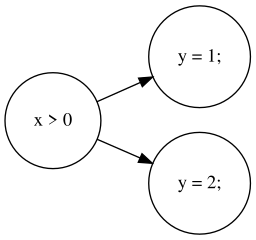
\includegraphics[width=0.5\textwidth]{Images/sample_edge_graph.png}
    \caption{Example of edge between basic blocks}
    \label{fig:sample_edge_graph}
\end{figure}
\phantom{}\\
When an edge is executed, the corresponding bit in the coverage map is incremented by \textit{+1} (to mark as ``\textit{hitted}"). The fuzzer uses this information to guide the generation of new test cases that maximize the coverage.
\\Within this action a coverage-guided fuzzer maintains a collection of inputs called \textbf{corpus}. In particular it is a collection of:
\begin{itemize}
    \item \textbf{Seeds}: Initial inputs that are used to start the fuzzing process.
    \item \textbf{Interesting inputs}: Inputs that are generated by the fuzzer during the fuzzing process and achieve new coverage (i.e. by mutating the seeds).
\end{itemize}
The corpus grows as the fuzzer adds new inputs that has allowed it to increase the coverage of the program.

\section{Stateful Fuzzing: Concepts and Challenges}
\textit{Stateless fuzzing} is a traditional fuzzing technique that generates random inputs to test the behavior of an application. However, this approach is not always effective for applications that maintain internal states across multiple interactions.
\\For example cosidering an FTP server, like \textbf{LightFTP} (\href{https://github.com/hfiref0x/LightFTP}{https://github.com/hfiref0x/LightFTP}), until the user is not authenticated, all the inputs are meaningless. In this case, the fuzzer should be able to generate a sequence of inputs that first authenticate the user and then test the behavior of the application.
\textit{Stateful fuzzing} adds state awareness to traditional fuzzing methods. It considers an application's internal state and how that state might affect subsequent inputs handling. This becomes particularly critical for applications that handle complex state information, such as network servers, databases and interactive applications.

\subsection{Understanding Stateful Applications}
Stateful applications maintain state across multiple interactions or sessions. Examples include network servers that manage connection states, authentication states, session identifiers, or other state information specific to an application. These states significantly influence the processing of inputs and the behavior of the application over time.
\\Good practices in state transition management are crucial for both security and reliability: bugs related to state transitions can lead to vulnerabilities such as unauthorized access, denial of service \textit{(DoS)}, or data corruption. 
\\Stateful fuzzers attempt to model and explore these state transitions by generating input sequences that mimic valid usage scenarios while concurrently monitoring state changes to ensure comprehensive coverage of all possible transitions. To better understand this concept, consider a simple state model shown in Figure \ref{fig:simplestatemodel}.
%TODO fix figure
\begin{figure}[h]
    \centering
    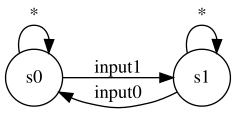
\includegraphics[width=0.5\textwidth]{Images/simplestatemodel.png}
    \caption{A simple state model illustrating state transitions in a stateful application}
    \label{fig:simplestatemodel}
\end{figure}


\subsection{Key Techniques in Stateful Fuzzing}
Stateful fuzzing involves several advanced techniques that distinguish it from traditional fuzzing approaches (\textit{The Art, Science, and Engineering of Fuzzing} \cite{theartoffuzzing}):

\begin{itemize}
    \item \textbf{State Modeling}: The process of building a model representing an application state machine by reverse engineering source code, observing real interactions, or guide test case generation in conjunction with machine learning techniques.
    
    \item \textbf{State Tracking}: This involves tracking the state of the application across successive inputs; indeed, tracking of network traffic, system calls, or internal state variables.
    
    \item \textbf{Feedback Mechanisms}: With feedback mechanisms, one can prioritize those test cases that tend to explore new states or code paths; hence, the general efficiency of fuzzing can be improved.
    
    \item \textbf{Sequence Generation}: It is the need to generate input sequences to properly model actual use, since the findings of vulnerabilities often depend on specific sequences or state transitions.
    
    \item \textbf{Learning-Based Approaches}: Certain fuzzers utilize machine learning or heuristic methodologies to dynamically ascertain the structural configuration of the application's state machine, thereby enabling the fuzzer to adjust and enhance its efficacy progressively.
\end{itemize}

\subsection{Challenges in Stateful Fuzzing}
Successfully performing testing is fraught with several challenges in stateful fuzzing (\textit{Is Stateful Fuzzing Really Challenging?} \cite{statefulfuzzingchallenges}):

\begin{itemize} 
    \item \textbf{State Explosion}: As in real life, an application itself may have a number of possible states and with more states, a risk for exponential growth in process complexity increases. In this case, state abstraction, pruning, or prioritization counters the \textit{state explosion} in an essential way.
    
    \item \textbf{Protocol Complexity}: Generating meaningful input sequences can involve deep knowledge of complex protocols or state machines. This often includes much domain-specific knowledge or even advanced algorithms.
    
    \item \textbf{Performance Overhead}: To date, state tracking performed by the application and input sequence generation can cause significant computational costs, hence slowing down the fuzzing process.

    \item \textbf{Handling Non-Deterministic Behavior}: The nondeterministic behavior of stateful applications often results from concurrency, differences in external inputs, or even timing variations. These factors therefore make the reproduction of bugs and receiving consistent fuzzing results usually difficult.

\end{itemize}

\section{Lighttpd: A Case Study for Stateful Fuzzing}
Lighttpd is an open-source web server optimized for performance with very low memory usage. It is designed to handle huge volumes of parallel connections with minimal overhead, making it particularly useful on systems with limited resources or those requiring a high degree of concurrency. Its modular design and support for advanced web protocols make it a popular choice for embedded systems, cloud computing platforms and high-traffic websites. It was used by popular websites like Wikimedia, YouTube and SourceForge, nowadays is used in general for ...%TODO add more

\subsection{Overview of Lighttpd Architecture}
Lighttpd operates on an event-driven architecture, which enables it to serve many requests concurrently. An asynchronous I/O framework is employed to minimize overhead in network connections, allowing the server to scale efficiently under varying workloads. The key features of Lighttpd include:

\begin{itemize}
    \item \textbf{Modular Design}: Provides a series of modules for implementing functions like \textit{URL rewriting}, \textit{HTTP compression}, \textit{SSL/TLS and WebSockets}. The modular design allows for customization based on specific needs.
    
    \item \textbf{Protocol Support}: Out of the box, it supports \textit{HTTP/1.1, HTTPS, FastCGI, SCGI and HTTP/2}, making it suitable for a wide range of web applications and services.
    
    \item \textbf{Security Attributes}: Advanced integrated security features include TLS/SSL encryption, prevention of \textit{denial-of-service} attacks and multiple authentication options.
\end{itemize}

\subsection{Relevance of Lighttpd for Fuzzing}

Lighttpd is an important SUT for fuzzing due to its common use behind various internet applications.
These characteristics make it a suitable candidate for evaluating fuzzing techniques.
By default, Lighttpd is maintains transient states during the processing of requests (Figure \ref{fig:lighttpdstatemodel}).
\begin{figure}[H]
    \centering
    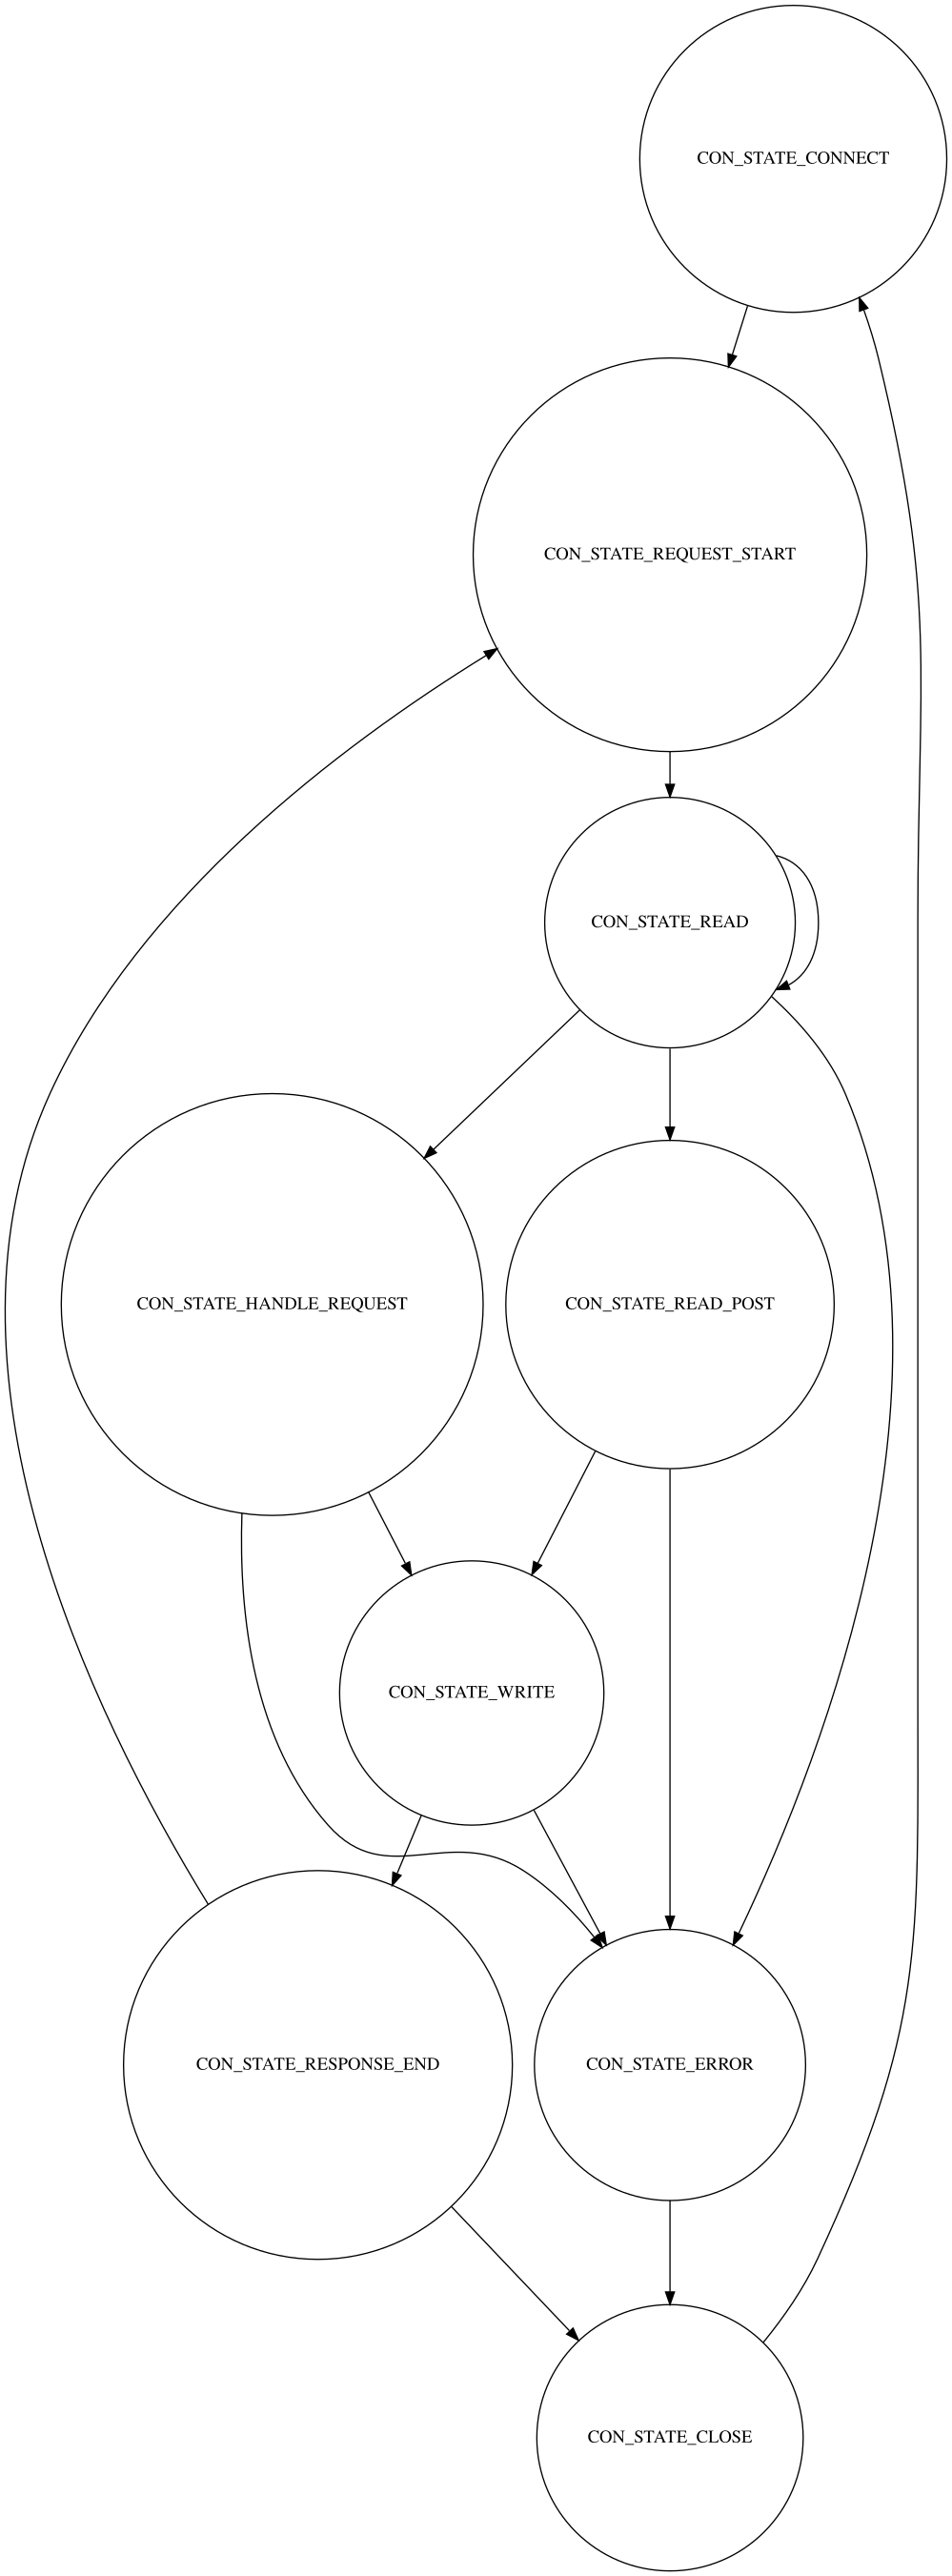
\includegraphics[width=0.6\textwidth]{Images/lighttpd_original.png}
    \caption{State model of Lighttpd}
    \label{fig:lighttpdstatemodel}
\end{figure}
\phantom{}\\
The state model seems to be complex, but the state are effectively transitory.
\\A sample flow of states in Lighttpd is as follows:
\begin{itemize}
    \item \textbf{1.CON\_STATE\_CONNECT}: The initial default state before a connection is established.
    
    \item \textbf{2.CON\_STATE\_REQUEST\_START}: The state right after a connection is established and wait for request.
    
    \item \textbf{3.CON\_STATE\_READ}: The state when the server is reading the request (here the server can be in a loop to read the request).
    
    \item \textbf{4.CON\_STATE\_HANDLE\_REQUEST}: The state when the server is processing the request, if body length is null.
    
    \item \textbf{4.CON\_STATE\_READ\_POST}: The state when the server is processing the request, if body length is more than 0.
    
    \item \textbf{5.CON\_STATE\_WRITE}: The state when the server is writing the response.
    \item \textbf{6.CON\_STATE\_ERROR}: The state when an unhandled error occurs.
    
    \item \textbf{7.CON\_STATE\_RESPONSE\_END}: The state after the request has been fully received.
    
    \item \textbf{8.CON\_STATE\_CLOSE}: The state when the connection is closed.
\end{itemize}
In the \textit{CON\_STATE\_CONNECT} ther is no control of input, because it only changes when the connection is established.
\\The only stationary state could be the \textit{CON\_STATE\_READ}, because it is a loop that reads the request (i.e. if the request is sent line by line, it will loop into it).
\\The other states are transitory because, at the end, it will go back to \textit{CON\_STATE\_REQUEST\_START} or \textit{CON\_STATE\_CONNECT}.
\\For this thesis, it has been chosen to model the state of the server based on the existence or non-existence of a resources (Figure \ref{fig:existent_nonexistent_resource_statemodel}). A resource can be a file, a directory, or any other entity that can be accessed via HTTP. By considering two types of requests—those that attempt to access an existing resource and those that attempt to access a non-existing resource—it can effectively explore different states of the server.

\section{Fuzzers Overview: AFLNet, ChatAFL and Fallaway}

For this thesis, three stateful fuzzers—AFLNet, ChatAFL and Fallaway—will be benchmarked over Lighttpd.
 
\subsection{AFLNet}
AFLNet \cite{AFLNet} is a stateful CGF tool. It integrates automated state model inference with coverage-guided fuzzing, creating a synergistic relationship between the two processes. As fuzzing generates new message sequences to reach unexplored states, it progressively builds a more complete state model. Concurrently, this dynamically evolving state model helps guide fuzzing efforts towards more significant areas of the code, leveraging both state and code coverage information of the retained message sequences.
\\AFLNet is implemented as an extension of the popular grey-box fuzzer AFL, with the additional capability of facilitating \textit{network communication} over sockets, which is not supported by the original AFL. To achieve this, AFLNet establishes two communication channels: one for sending messages to the SUT and another for receiving responses. The response-receiving channel acts as a state feedback channel, complementing the code coverage feedback channel utilized by other CGF tools. The communication is implemented using standard C Socket APIs and synchronization between AFLNet and the server is ensured by introducing delays between requests.
\\AFLNet uses a \textit{prefix-based fuzzing} strategy, where the fuzzer maintains a prefix of the message sequence that has been successfully processed by the server. This prefix is used to guide the generation of new message sequences, ensuring that the fuzzer explores new states and code paths while maintaining the validity of the input.
\\The seeds to AFLNet consists of \textit{pcap} files capturing network traffic, such as interactions between a client and server. A network sniffer, like \textit{tcpdump}, is used to capture realistic exchanges and a packet analyzer, such as Wireshark, can automatically extract the relevant message sequences. AFLNet uses a \textbf{Request Sequence Parser} to generate an initial corpus of message sequences by parsing these pcap files. It isolates individual client requests, discards the responses and identifies the beginning and end of each message, utilizing protocol-specific markers.
\\The \textbf{State Machine Learner} component then augments the protocol state machine with newly observed states and transitions by analyzing server responses. AFLNet extracts status codes from server responses to identify and document new states and transitions. The \textbf{Target State Selector} leverages this information to determine which state the fuzzer should focus on next. This is done by applying several heuristics based on the statistical data gathered from the state machine, aiming to identify ``blind spots" or rarely exercised states and maximize the discovery of new state transitions.
\\Once a target state is selected, the \textbf{Sequence Selector} chooses a corresponding message sequence from the corpus that can reach the desired state. AFLNet maintains a state corpus and a hashmap to facilitate efficient selection of sequences. The selected sequence is then subjected to mutation using the \textbf{Sequence Mutator}, which builds upon AFL's \textit{`fuzz\_one`} method (\textit{input selection, mutation, execution, feedback collecltion, minimization and prioritization, looping}). AFLNet uses \textit{protocol-aware} mutation operators to modify the candidate subsequence, enhancing the chances of generating new sequences that can lead to the discovery of new states or code branches.
\\AFLNet employs several mutation strategies, such as replacing, inserting, duplicating, or deleting messages, in addition to standard byte-level operations like bit flipping. Generated sequences deemed ``interesting" — those that uncover new states, transitions, or code branches — are added to the corpus for further fuzzing. This evolutionary approach, driven by the continuous enhancement of the message sequence corpus, underpins the effectiveness of AFLNet in achieving comprehensive state and code coverage.

\subsection{ChatAFL}
Traditional \textit{mutation-based protocol fuzzing} relies heavily on recorded message sequences to generate test cases, which can limit its effectiveness in thoroughly exploring the input and state space of complex network protocols. Existing approaches often require detailed, \textit{machine-readable} protocol specifications, which are labor-intensive to produce and maintain. Furthermore, these approaches may struggle with limited seed diversity and may reach a coverage plateau (no more progress in discovering code paths or states), where further exploration yields diminishing returns.
\\To address these limitations, recent advancements have explored the potential of \textit{Large Language Models (LLMs)} \cite{minaee2024largelanguagemodelssurvey} to assist in the fuzzing process.
\\LLMs are a class of neural network models that have demonstrated remarkable capabilities in natural language understanding and generation. They can be fine-tuned for specific tasks and have been successfully applied to a wide range of applications, including language translation, text generation and code completion.
\\LLMs are pre-trained on extensive corpora, including publicly available protocol specifications and have demonstrated impressive capabilities in understanding and generating text. This presents an opportunity to leverage LLMs to improve fuzzing strategies by interpreting natural language descriptions of protocols and generating structured, diverse message sequences.
\\\textit{LLM-guided protocol fuzzing} uses the capabilities of LLMs to overcome the limitations of traditional mutation-based fuzzers. This method is implemented in ChatAFL \cite{chatafl} , a fuzzing tool built upon the AFLNet framework. ChatAFL incorporates LLMs to assist in three key areas:

\begin{enumerate}
    \item \textbf{Grammar Extraction:} By querying the LLM, the fuzzer can obtain a machine-readable grammar for the protocol under test. This grammar is used to guide mutations in a way that maintains the structural validity of the messages, thus enhancing the fuzzer's ability to explore new state transitions.

    \item \textbf{Seed Enrichment:} The LLM is used to diversify the initial seed corpus by generating new message types that are contextually relevant to the protocol. This helps to overcome the limitations posed by a narrow set of initial test cases and increases the likelihood of discovering new protocol behaviors.

    \item \textbf{Breaking Coverage Plateaus:} When the fuzzer is unable to achieve further state or code coverage, it is considered to be in a coverage plateau. The LLM can be prompted to generate new message sequences aimed at escaping the plateau by triggering unexplored state transitions.
\end{enumerate}
The integration of LLMs into protocol fuzzing offers several benefits:
\begin{enumerate}
    \item It reduces the dependence on pre-existing machine-readable protocol specifications by leveraging natural language processing capabilities.
    \item It enhances the diversity and effectiveness of the fuzzing process by generating a wider variety of input sequences.
    \item It aligns with the inherent goals of fuzzing — automation and adaptability — by using LLMs that can be easily guided via prompts to perform specific tasks without extensive reprogramming or manual intervention.
\end{enumerate}
Overall, this LLM-guided approach, as demonstrated in ChatAFL, represents a novel direction in protocol fuzzing, combining traditional techniques with \textit{state-of-the-art} language models to improve both the breadth and depth of fuzzing campaigns.


\subsection{Fallaway}
Fallaway \cite{Fallaway} is a stateful fuzzer designed to address several key challenges faced by traditional fuzzers when handling stateful SUTs. Unlike stateless fuzzers such as AFL, which send single test cases and expect the SUT to terminate, Fallaway manages multiple states by incorporating a \textit{dual-loop} structure: an outer loop that selects the SUT state and an inner loop that sends multiple test cases for the chosen state. This approach helps maintain deliberate focus on specific states, prevents interference between states and ensures that progress in one state does not hinder progress in another.
\\To achieve these objectives, Fallaway decouples the concepts of state scheduling and test case (seed) scheduling.
The fuzzer has a \textbf{queue}, that is a scheduling algorithm that selects the next input to use based on different strategies like:
\begin{itemize}
    \item \textbf{Coverage-Yield (CY)} strategy, which uses a round-robin approach to select the next input to mutate.
    \item \textbf{Outgoing Edges (OE)} strategy, which prioritizes inputs that exercise new edges in the program (this is done by using metadata that keeps track of the outgoing edges of each state in the program and selecting the input that exercises the most new edges).
\end{itemize} 
Corpus and queue are used interchangeably, but they are not really the same thing. \\We can look at the queue as a mapping of the corpus within a scheduling algorithm to choose the next input to mutate.
\\These are some examples of coverage-guided strategies:
\begin{itemize}
    \item \textbf{Multiple Corpus Single Map (MCSM)}: This strategy uses a single coverage map to track the coverage of the program and multiple queues to store the inputs (is more efficient in terms of memory usage and faster in terms of execution time, but it is less effective in terms of coverage).
    
    \item \textbf{Multiple Corpus Multiple Map (MCMM)}: This strategy uses multiple coverage maps to track the coverage of the program and multiple queues to store the inputs (is more effective in terms of coverage, but it is less efficient in terms of memory usage and slower in terms of execution time).
\end{itemize}
Each queue contains inputs that have allowed the fuzzer to reach a specific state of the program. The fuzzer uses a scheduler to select which input to mutate next based on the coverage achieved by the input.
\\For each state, a unique prefix is maintained along with a separate corpus of test cases, allowing focused exploration of the SUT's behavior within that state. Observations and feedback are also stored separately for each state, avoiding the problem of feedback contamination across different states. This strategy enables the fuzzer to maintain a clear distinction between the information gathered in each state, ensuring that the testing process remains unbiased and effective.
\\Fallaway is built on the \textbf{LibAFL} \cite{libafl} framework, which is a modular library for developing fuzzers. To make LibAFL suitable for stateful SUTs, Fallaway extends its functionality in two key ways:
\begin{enumerate}
    \item It uses AFL's \textbf{persistent mode}, designed to keep a SUT application running continuously between different test cases, rather than starting a new process for each test case. This approach is particularly useful for maintaining and manipulating the application's state across test cases, allowing the SUT to handle inputs continuously without resetting after each test case, which is crucial for efficient fuzzing of stateful systems.
    \item It introduces an outer loop to handle state transitions and reset the SUT accordingly, ensuring compatibility with LibAFL's existing mechanisms for executing test cases.
\end{enumerate}  
By integrating these methods, Fallaway leverages the speed and efficiency of persistent mode fuzzing while maintaining precise control over state transitions. This approach allows it balance execution speed and focus state exploration.
